\begin{frame}
  \scriptsize{\tableofcontents}
\end{frame}

\section{Jogos}
\subsection{História}

\AtBeginSection[]
{
  \begin{frame}<beamer>
    \scriptsize{\tableofcontents[currentsection]}
  \end{frame}
}

\myframe{
  \begin{center}
    \includegraphics[height=0.8\textheight]{img/collage.jpg}
  \end{center}
}

\myframe{
  \ctr{Introdução}
  \begin{itemize}
    \item Desde, pelo menos, 2600 AC;
    \item Alguns sofreram poucas alterações em 2000 anos;
    \item Chegaram ao \emph{mainstream};
    \item Aplicações na economia, computação, matemática e pedagogia.
    \item Recreação; Estudos de comportamento; Gamificação; Ensino; Esportes;
      Desafios; Puzzles;
  \end{itemize}
}

\section{Inteligência Artificial em Jogos}

\subsection{Introdução}

\myframe{
  \ctr{Inteligência Artificial}
  \begin{itemize}
    \item Replicação de um humano;
    \item Limitações computacionais;
    \item Limitações humanas;
    \item Várias aplicações;
    \item Interesse antigo.
  \end{itemize}
}

\subsection{IA em Jogos}

\myframe{
  \ctr{IA em Jogos}
  \begin{itemize}
    \item Diversão e desafio;
    \item Pacman;
    \item Lógica;
    \item Solução básica: Força bruta;
  \end{itemize}
}

\myframe{
  \begin{center}
    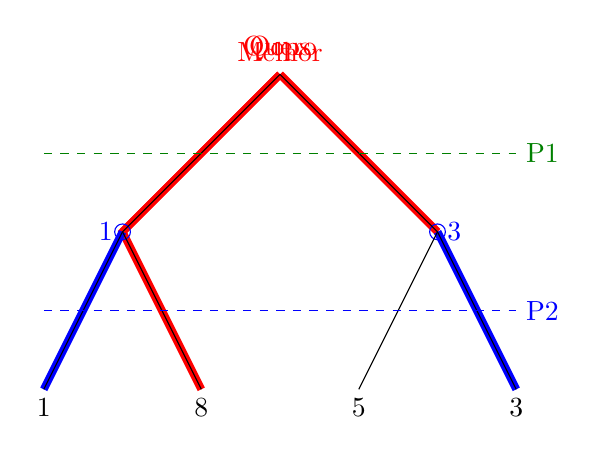
\begin{tikzpicture}
    \onslide<2>{
      \draw[red, line width=1.0mm] (0,0) node[above] {Quero} -- (-2,-2) --
        (-1,-4);
    }
    \onslide<3>{
      \draw[red, line width=1.0mm] (0,0) node[above] {Oops} -- (-2,-2);
      \draw[blue, line width=1.0mm] (-2,-2) -- (-3,-4);
    }
    \onslide<4>{
      \draw[red, line width=1.0mm] (0,0) node[above] {Melhor} -- (2,-2);
      \draw[blue, line width=1.0mm] (2,-2) -- (3,-4);
    }
    \onslide<5>{
      \draw[blue] (2,-2) circle[radius=0.1] node[right] {3};
      \draw[blue] (-2,-2) circle[radius=0.1] node[left] {1};
    }
      \draw (0,0) -- (2,-2);
      \draw (0,0) -- (-2,-2);
      \draw (2,-2) -- (3,-4) node[below] {3};
      \draw (2,-2) -- (1,-4) node[below] {5};
      \draw (-2,-2) -- (-3,-4) node[below] {1};
      \draw (-2,-2) -- (-1,-4) node[below] {8};
      \draw[dashed,green!50!black] (-3,-1) -- (3,-1) node[right] {P1};
    \onslide<1-4>{
      \draw[dashed,blue] (-3,-3) -- (3,-3) node[right] {P2};
    }
    \end{tikzpicture}
  \end{center}
}

\myframe{
  \begin{center}
    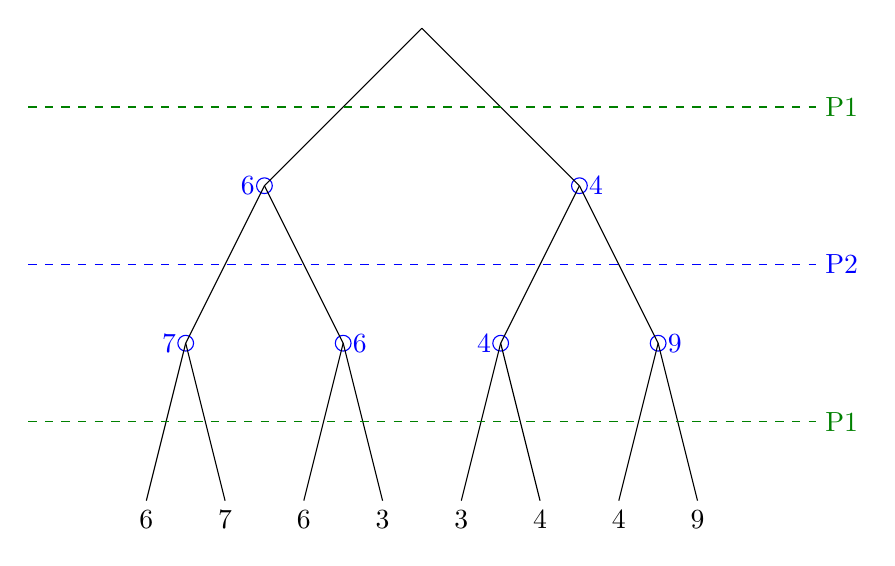
\begin{tikzpicture}
    \onslide<2-3>{
      \draw[blue] (3,-4) circle[radius=0.1] node[right] {9};
      \draw[blue] (1,-4) circle[radius=0.1] node[left] {4};
      \draw[blue] (-3,-4) circle[radius=0.1] node[left] {7};
      \draw[blue] (-1,-4) circle[radius=0.1] node[right] {6};
    }
    \onslide<3>{
      \draw[blue] (2,-2) circle[radius=0.1] node[right] {4};
      \draw[blue] (-2,-2) circle[radius=0.1] node[left] {6};
    }
      \draw (0,0) -- (2,-2);
      \draw (0,0) -- (-2,-2);
      \draw (2,-2) -- (3,-4);
      \draw (2,-2) -- (1,-4);
      \draw (-2,-2) -- (-3,-4);
      \draw (-2,-2) -- (-1,-4);
      \draw (3,-4) -- (3.5,-6) node[below] {9};
      \draw (3,-4) -- (2.5,-6) node[below] {4};
      \draw (-3,-4) -- (-3.5,-6) node[below] {6};
      \draw (-3,-4) -- (-2.5,-6) node[below] {7};
      \draw (1,-4) -- (0.5,-6) node[below] {3};
      \draw (1,-4) -- (1.5,-6) node[below] {4};
      \draw (-1,-4) -- (-1.5,-6) node[below] {6};
      \draw (-1,-4) -- (-0.5,-6) node[below] {3};
      \draw[dashed,green!50!black] (-5,-1) -- (5,-1) node[right] {P1};
      \draw[dashed,blue] (-5,-3) -- (5,-3) node[right] {P2};
      \draw[dashed,green!50!black] (-5,-5) -- (5,-5) node[right] {P1};
    \end{tikzpicture}
  \end{center}
}

\myframe{
\begin{center}
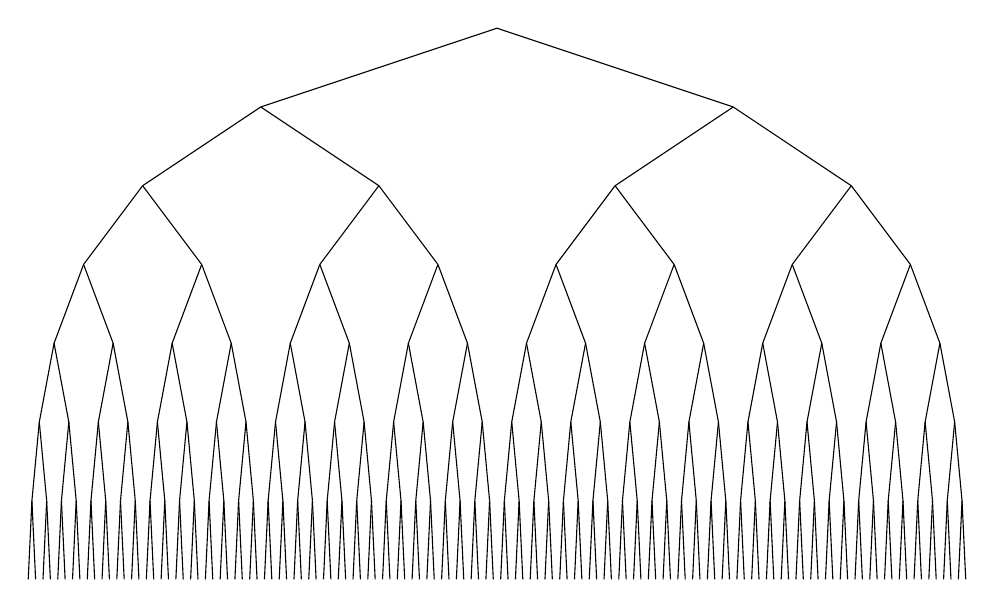
\begin{tikzpicture}
\def\L{12}
\foreach \j in {0,...,6} {
	\pgfmathsetmacro{\Ni}{pow(2,\j)}
	\foreach \i in {1,...,\Ni} {
		\pgfmathsetmacro{\x}{(\i - (\Ni+1)/2)*\L/\Ni}
		\pgfmathsetmacro{\h}{\L/4/\Ni}
		\pgfmathsetmacro{\y}{-\j}
		\pgfmathsetmacro{\yp}{-\j-1}
		\draw (\x,\y) -- ({\x+\h},\yp);
		\draw (\x,\y) -- ({\x-\h},\yp);
	}
}
\end{tikzpicture}
\end{center}
}

\myframe{
\begin{center}
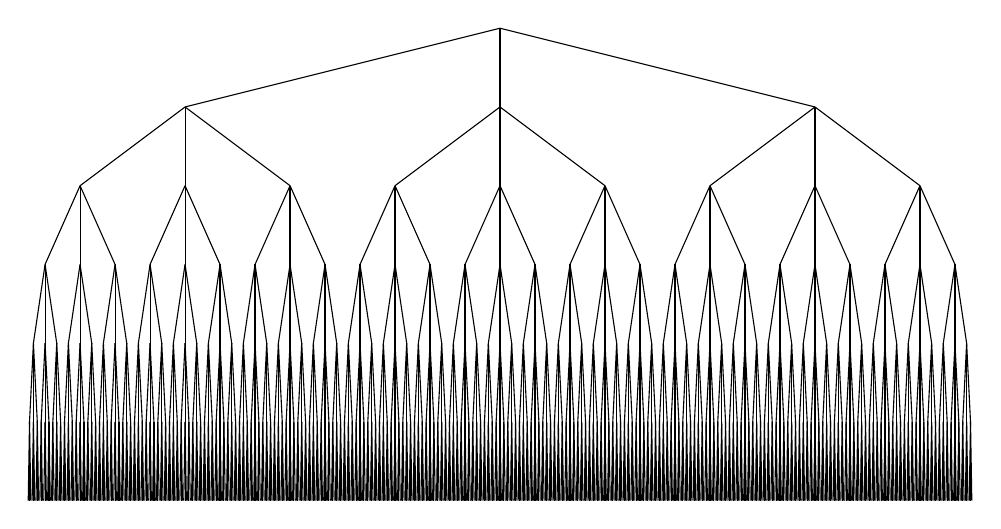
\begin{tikzpicture}
\def\L{12}
\foreach \j in {0,...,5} {
	\pgfmathsetmacro{\Ni}{pow(3,\j)}
	\foreach \i in {1,...,\Ni} {
		\pgfmathsetmacro{\x}{(\i - (\Ni+1)/2)*\L/\Ni}
		\pgfmathsetmacro{\h}{\L/3/\Ni}
		\pgfmathsetmacro{\y}{-\j}
		\pgfmathsetmacro{\yp}{-\j-1}
		\draw (\x,\y) -- ({\x},\yp);
		\draw (\x,\y) -- ({\x+\h},\yp);
		\draw (\x,\y) -- ({\x-\h},\yp);
	}
}
\end{tikzpicture}
\end{center}
}

\myframe{
\begin{center}
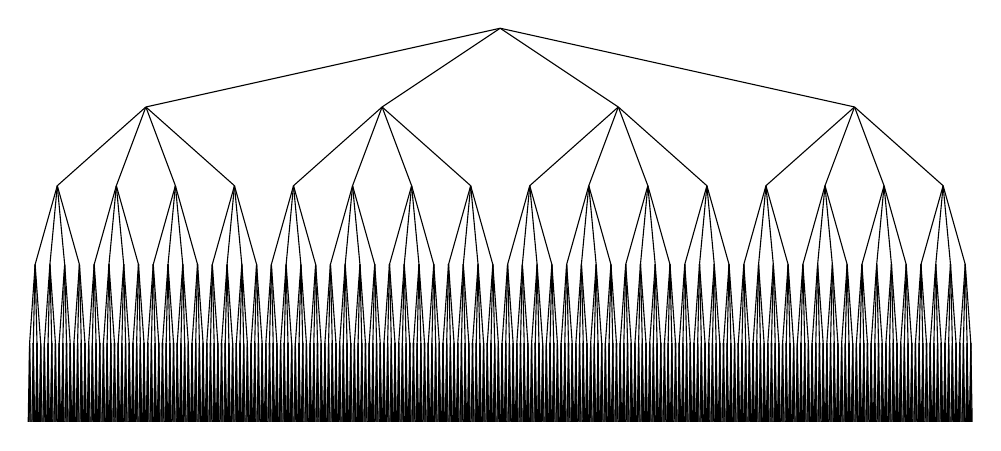
\begin{tikzpicture}
\def\L{12}
\foreach \j in {0,...,4} {
	\pgfmathsetmacro{\Ni}{pow(4,\j)}
	\foreach \i in {1,...,\Ni} {
		\pgfmathsetmacro{\x}{(\i - (\Ni+1)/2)*\L/\Ni}
		\pgfmathsetmacro{\h}{\L/4/\Ni}
		\pgfmathsetmacro{\y}{-\j}
		\pgfmathsetmacro{\yp}{-\j-1}
		\draw (\x,\y) -- ({\x+3*\h/2},\yp);
		\draw (\x,\y) -- ({\x-3*\h/2},\yp);
		\draw (\x,\y) -- ({\x+\h/2},\yp);
		\draw (\x,\y) -- ({\x-\h/2},\yp);
	}
}
\end{tikzpicture}
\end{center}
}

\subsection{Jogo da velha}

\newcommand{\cross}[1]{
  \draw[red,line width=2.0mm,shift={#1}] (-0.7,-0.7) -- (0.7,0.7);
  \draw[red,line width=2.0mm,shift={#1}] (0.7,-0.7) -- (-0.7,0.7);
}
\newcommand{\nought}[1]{
  \draw[blue,line width=2.0mm,shift={#1}] (0,0) circle[radius=0.6];
}

\myframe{
  \begin{center}
    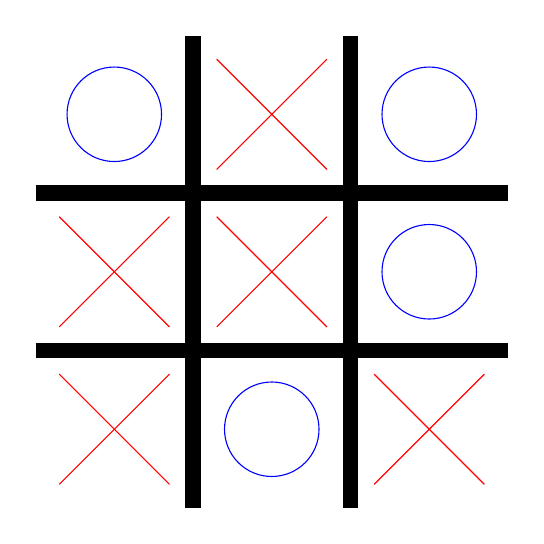
\begin{tikzpicture}
      \draw[line width=2.0mm] (-1,-3) -- (-1,3);
      \draw[line width=2.0mm] (1,-3) -- (1,3);
      \draw[line width=2.0mm] (-3,-1) -- (3,-1);
      \draw[line width=2.0mm] (-3,1) -- (3,1);
\onslide<2->{ \cross{(0,0)} }
\onslide<3->{ \nought{(2,2)} }
\onslide<4->{ \cross{(2,-2)} }
\onslide<5->{ \nought{(-2,2)} }
\onslide<6->{ \cross{(0,2)} }
\onslide<7->{ \nought{(0,-2)} }
\onslide<8->{ \cross{(-2,0)} }
\onslide<9->{ \nought{(2,0)} }
\onslide<10->{ \cross{(-2,-2)} }
    \end{tikzpicture}
  \end{center}
}

\renewcommand{\cross}[1]{
  \draw[red,shift={#1}] (-0.7,-0.7) -- (0.7,0.7);
  \draw[red,shift={#1}] (0.7,-0.7) -- (-0.7,0.7);
}
\renewcommand{\nought}[1]{
  \draw[blue,shift={#1}] (0,0) circle[radius=0.6];
}

\myframe{
\begin{center}
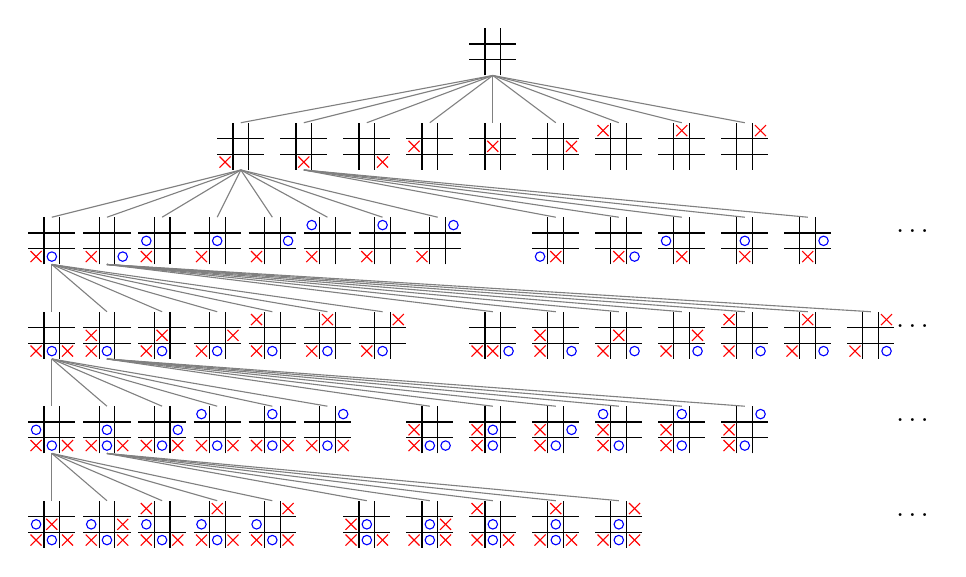
\begin{tikzpicture}[scale=0.1]
  \draw (-1,-3) -- (-1,3);
  \draw (1,-3) -- (1,3);
  \draw (-3,-1) -- (3,-1);
  \draw (-3,1) -- (3,1);
  \pause
  % Level 1
  \def\y{-12}
  \foreach \k in {1,2,...,9} {
    \pgfmathsetmacro{\x}{8*(\k-5)}
    \draw[gray] (0,-3) -- (\x,{\y+3});
    \draw[shift={(\x,\y)}] (-1,-3) -- (-1,3);
    \draw[shift={(\x,\y)}] (1,-3) -- (1,3);
    \draw[shift={(\x,\y)}] (-3,-1) -- (3,-1);
    \draw[shift={(\x,\y)}] (-3,1) -- (3,1);
    \pgfmathsetmacro{\i}{-2+mod(\k-1,3)*2}
    \pgfmathsetmacro{\j}{-2+int((\k-1)/3)*2}
    \cross{({\x+\i},{\y+\j})}
  }
  \pause
  % Level 2
  \def\yold{-12}
  \def\y{-12*2}
  \foreach \k in {2,...,9} {
    \pgfmathsetmacro{\x}{7*(\k-10)}
    \draw[gray] ({-4*8},{\yold-3}) -- (\x,{\y+3});
    \draw[shift={(\x,\y)}] (-1,-3) -- (-1,3);
    \draw[shift={(\x,\y)}] (1,-3) -- (1,3);
    \draw[shift={(\x,\y)}] (-3,-1) -- (3,-1);
    \draw[shift={(\x,\y)}] (-3,1) -- (3,1);
    \pgfmathsetmacro{\i}{-2+mod(\k-1,3)*2}
    \pgfmathsetmacro{\j}{-2+int((\k-1)/3)*2}
    \cross{({\x-2},{\y-2})}
    \nought{({\x+\i},{\y+\j})}
  }
  \foreach \k in {1,3,4,5,6} {
    \pgfmathsetmacro{\x}{ifthenelse(\k<2, 8*(\k), 8*(\k-1)}
    \draw[gray] ({-3*8},{\yold-3}) -- (\x,{\y+3});
    \draw[shift={(\x,\y)}] (-1,-3) -- (-1,3);
    \draw[shift={(\x,\y)}] (1,-3) -- (1,3);
    \draw[shift={(\x,\y)}] (-3,-1) -- (3,-1);
    \draw[shift={(\x,\y)}] (-3,1) -- (3,1);
    \pgfmathsetmacro{\i}{-2+mod(\k-1,3)*2}
    \pgfmathsetmacro{\j}{-2+int((\k-1)/3)*2}
    \cross{({\x},{\y-2})}
    \nought{({\x+\i},{\y+\j})}
  }
  \draw ({10*5},{-12*1.9}) node[right] {$\dots$};
  \pause
  % Level 3
  \def\yold{-12*2}
  \def\y{-12*3}
  \foreach \k in {3,...,9} {
    \pgfmathsetmacro{\x}{7*(\k-11)}
    \draw[gray] ({-8*7},{\yold-3}) -- (\x,{\y+3});
    \draw[shift={(\x,\y)}] (-1,-3) -- (-1,3);
    \draw[shift={(\x,\y)}] (1,-3) -- (1,3);
    \draw[shift={(\x,\y)}] (-3,-1) -- (3,-1);
    \draw[shift={(\x,\y)}] (-3,1) -- (3,1);
    \pgfmathsetmacro{\i}{-2+mod(\k-1,3)*2}
    \pgfmathsetmacro{\j}{-2+int((\k-1)/3)*2}
    \cross{({\x-2},{\y-2})}
    \nought{(\x,{\y-2})}
    \cross{({\x+\i},{\y+\j})}
  }
  \foreach \k in {2,4,5,6,...,9} {
    \pgfmathsetmacro{\x}{ifthenelse(\k<3, 8*(\k-2), 8*(\k-3)}
    \draw[gray] ({-7*7},{\yold-3}) -- (\x,{\y+3});
    \draw[shift={(\x,\y)}] (-1,-3) -- (-1,3);
    \draw[shift={(\x,\y)}] (1,-3) -- (1,3);
    \draw[shift={(\x,\y)}] (-3,-1) -- (3,-1);
    \draw[shift={(\x,\y)}] (-3,1) -- (3,1);
    \pgfmathsetmacro{\i}{-2+mod(\k-1,3)*2}
    \pgfmathsetmacro{\j}{-2+int((\k-1)/3)*2}
    \cross{({\x-2},{\y-2})}
    \nought{({\x+2},{\y-2})}
    \cross{({\x+\i},{\y+\j})}
  }
  \draw ({10*5},{-12*2.9}) node[right] {$\dots$};
  \pause
  % Level 4
  \def\yold{-12*3}
  \def\y{-12*4}
  \foreach \k in {4,...,9} {
    \pgfmathsetmacro{\x}{7*(\k-12)}
    \draw[gray] ({-8*7},{\yold-3}) -- (\x,{\y+3});
    \draw[shift={(\x,\y)}] (-1,-3) -- (-1,3);
    \draw[shift={(\x,\y)}] (1,-3) -- (1,3);
    \draw[shift={(\x,\y)}] (-3,-1) -- (3,-1);
    \draw[shift={(\x,\y)}] (-3,1) -- (3,1);
    \pgfmathsetmacro{\i}{-2+mod(\k-1,3)*2}
    \pgfmathsetmacro{\j}{-2+int((\k-1)/3)*2}
    \cross{({\x-2},{\y-2})}
    \nought{(\x,{\y-2})}
    \cross{({\x+2},{\y-2})}
    \nought{({\x+\i},{\y+\j})}
  }
  \foreach \k in {3,5,6,...,9} {
    \pgfmathsetmacro{\x}{ifthenelse(\k<4, 8*(\k-4), 8*(\k-5)}
    \draw[gray] ({-7*7},{\yold-3}) -- (\x,{\y+3});
    \draw[shift={(\x,\y)}] (-1,-3) -- (-1,3);
    \draw[shift={(\x,\y)}] (1,-3) -- (1,3);
    \draw[shift={(\x,\y)}] (-3,-1) -- (3,-1);
    \draw[shift={(\x,\y)}] (-3,1) -- (3,1);
    \pgfmathsetmacro{\i}{-2+mod(\k-1,3)*2}
    \pgfmathsetmacro{\j}{-2+int((\k-1)/3)*2}
    \cross{({\x-2},{\y-2})}
    \nought{(\x,{\y-2})}
    \cross{({\x-2},{\y})}
    \nought{({\x+\i},{\y+\j})}
  }
  \draw ({10*5},{-12*3.9}) node[right] {$\dots$};
  \pause
  % Level 5
  \def\yold{-12*4}
  \def\y{-12*5}
  \foreach \k in {5,...,9} {
    \pgfmathsetmacro{\x}{7*(\k-13)}
    \draw[gray] ({-8*7},{\yold-3}) -- (\x,{\y+3});
    \draw[shift={(\x,\y)}] (-1,-3) -- (-1,3);
    \draw[shift={(\x,\y)}] (1,-3) -- (1,3);
    \draw[shift={(\x,\y)}] (-3,-1) -- (3,-1);
    \draw[shift={(\x,\y)}] (-3,1) -- (3,1);
    \pgfmathsetmacro{\i}{-2+mod(\k-1,3)*2}
    \pgfmathsetmacro{\j}{-2+int((\k-1)/3)*2}
    \cross{({\x-2},{\y-2})}
    \nought{(\x,{\y-2})}
    \cross{({\x+2},{\y-2})}
    \nought{({\x-2},{\y})}
    \cross{({\x+\i},{\y+\j})}
  }
  \foreach \k in {4,6,7,8,9} {
    \pgfmathsetmacro{\x}{ifthenelse(\k<5, 8*(\k-6), 8*(\k-7)}
    \draw[gray] ({-7*7},{\yold-3}) -- (\x,{\y+3});
    \draw[shift={(\x,\y)}] (-1,-3) -- (-1,3);
    \draw[shift={(\x,\y)}] (1,-3) -- (1,3);
    \draw[shift={(\x,\y)}] (-3,-1) -- (3,-1);
    \draw[shift={(\x,\y)}] (-3,1) -- (3,1);
    \pgfmathsetmacro{\i}{-2+mod(\k-1,3)*2}
    \pgfmathsetmacro{\j}{-2+int((\k-1)/3)*2}
    \cross{({\x-2},{\y-2})}
    \nought{(\x,{\y-2})}
    \cross{({\x+2},{\y-2})}
    \nought{({\x},{\y})}
    \cross{({\x+\i},{\y+\j})}
  }
  \draw ({10*5},{-12*4.9}) node[right] {$\dots$};
\end{tikzpicture}
\end{center}
}

\myframe{
  \ctr{Jogo da velha}
  \begin{itemize}
    \item $9! = 362880$ jogos.
    \item Mesmo assim um computador consegue realizar a verificação necessária
      para nunca perder, desde 1952.
    \item Na prática, rotações e reflexões diminuem essa quantidade para
      26830 jogos possíveis.
  \end{itemize}
}

\subsection{Xadrez}

\myframe{
  \ctr{Xadrez}
  \begin{itemize}
    \item $\approx 10^{124}$ jogos
    \item Impraticável (ou impossível) ver todos os jogos
    \item Ainda assim, em 1996, \emph{Deep Blue} venceu o primeiro jogo
      contra Garry Kasparov (perdeu 3 e empatou 2). Em 1997, Deep Blue empatou 5
      e venceu 1. Deep Blue analisava até $2\times10^8$ posições por segundo.
    \item Hoje, é muito mais fácil um computador conseguir o empate.
  \end{itemize}
}

\myframe{
  \ctr{Como?}
  \begin{itemize}
    \item Banco de dados de aberturas
    \item Lógica de fim de jogo
    \item Avaliação de posições
    \item Heurísticas de buscas
  \end{itemize}
}

\subsection{Go}

\myframe{
  \ctr{Go}
  \begin{itemize}
    \item 2500 anos.
    \item Uma das ``quatro artes''.
    \item $\approx 10^{170}$ posições válidas.
    \item Por baixo, $\approx 10^{336}$ (de umas 150 jogadas, com uma 250
      opções).
    \item $361! \approx 10^{768}$
  \end{itemize}
}

\myframe{
  \ctr{Muito mais difícil}
  \begin{itemize}
    \item Muito mais possibilidades
    \item As repercussões são maiores
    \item Uma estratégia local pode não ser boa globalmente
    \item Não é fácil avaliar uma posição
    \item<2> Março de 2016: \emph{DeepMind} vence Lee Seidol, 4 a 1.
  \end{itemize}
}

\section{Teoria}

\subsection{Múltiplas máquinas caça-níquel}

\myframe{
	\ctr{Múltiplas máquinas caça-níquel ou {\it multi-armed bandit}}
	\begin{itemize}
    \item Número finito de máquinas ($K$)
    \item A esperança de retorno é desconhecida
    \item Estimativa ($R_j$ retorno, $n_j$ número de jogadas).
      \[ \mu_j = \frac{1}{n_j}\sum_{i = 1}^{n_j}R_j \]
	\end{itemize}
}

\myframe{
\begin{center}
\begin{tikzpicture}
  \only<1>{
  \node[draw,circle] (d6) at (-3,0) {Dado d6};
  \node[draw,circle] (d12) at (0,0) {Dado d12};
  \node[draw,circle] (d20) at (3,0) {Dado d20};
  }
  \onslide<2->{
  \node[draw,circle,fill=black!90!white] (d6) at (-3,0) {Dado d6};
  \node[draw,circle,fill=black!90!white] (d12) at (0,0) {Dado d12};
  \node[draw,circle,fill=black!90!white] (d20) at (3,0) {Dado d20};
  }
  \onslide<3->{
  \node[below of=d6,node distance=4em] (d6j1) {6};
  \node[below of=d12,node distance=4em] (d12j1) {5};
  \node[below of=d20,node distance=4em] (d20j1) {4};
  }
  \onslide<4->{
  \node[below of=d6j1,node distance=2em] (d6j2) {3};
  }
  \onslide<5->{
  \node[below of=d12j1,node distance=2em] (d12j2) {8};
  }
  \onslide<6->{
  \node[below of=d12j2,node distance=2em] (d12j3) {1};
  }
  \onslide<7->{
  \node[below of=d12j3,node distance=2em] (d12j4) {2};
  }
  \onslide<8->{
  \node[below of=d6j2,node distance=2em] (d6j3) {3};
  }
  \foreach \p [count=\i] in {3.5, ?, 6, 4.5, 4.5, 4.5, 4.5, 4} {
    \only<\i>{\node[above of=d6, node distance=4em] (mu1) {$\mu_1 = \p$};}
  }
  \foreach \n [count=\i] in {-, 0, 1, 2, 2, 2, 2, 3} {
    \only<\i>{\node[above of=mu1, node distance=2em] (n1) {$N_1 = \n$};}
  }
  \foreach \p [count=\i] in {6.5, ?, 5, 5, 6.5, 4.67, 4, 4} {
    \only<\i>{\node[above of=d12, node distance=4em] (mu2) {$\mu_2 = \p$};}
  }
  \foreach \n [count=\i] in {-, 0, 1, 1, 2, 3, 4, 4} {
    \only<\i>{\node[above of=mu2, node distance=2em] (n2) {$N_2 = \n$};}
  }
  \foreach \p [count=\i] in {10.5, ?, 4, 4, 4, 4, 4, 4} {
    \only<\i>{\node[above of=d20, node distance=4em] (mu3) {$\mu_3 = \p$};}
  }
  \foreach \n [count=\i] in {-, 0, 1, 1, 1, 1, 1, 1} {
    \only<\i>{\node[above of=mu3, node distance=2em] (n3) {$N_3 = \n$};}
  }
\end{tikzpicture}
\end{center}
}

\myframe{
  \ctr{Algoritmo UCB (Upper Confidence Bound)}
  \[ B_j = \left\{\begin{array}{ll}
    +\infty & n_j = 0 \\
    \mu_j + \sqrt{\dfrac{2\log(N)}{n_j}}, & n_j > 0
    \end{array}\right.  \]
  onde $\displaystyle N = \sum_{j=1}^K n_j$.
}

\myframe{
  \foreach \N [count=\i] in {-,0,3,4,5,6} {
    \only<\i>{ \ctr{N = \N} }
  }
\begin{center}
\begin{tikzpicture}
  \only<1>{
  \node[draw,circle] (d6) at (-3,0) {Dado d6};
  \node[draw,circle] (d12) at (0,0) {Dado d12};
  \node[draw,circle] (d20) at (3,0) {Dado d20};
  }
  \onslide<2->{
  \node[draw,circle,fill=black!90!white] (d6) at (-3,0) {Dado d6};
  \node[draw,circle,fill=black!90!white] (d12) at (0,0) {Dado d12};
  \node[draw,circle,fill=black!90!white] (d20) at (3,0) {Dado d20};
  }
  \onslide<3->{
  \node[below of=d6,node distance=4em] (d6j1) {6};
  \node[below of=d12,node distance=4em] (d12j1) {5};
  \node[below of=d20,node distance=4em] (d20j1) {4};
  }
  \onslide<4->{
  \node[below of=d6j1,node distance=1.5em] (d6j2) {3};
  }
  \onslide<5->{
  \node[below of=d12j1,node distance=1.5em] (d12j2) {8};
  }
  \onslide<6->{
  \node[below of=d12j2,node distance=1.5em] (d12j3) {1};
  }
  \foreach \p [count=\i] in {3.5, ?, 6, 4.5, 4.5, 4.5} {
    \only<\i>{\node[above of=d6, node distance=4em] (mu1) {$\mu_1 = \p$};}
  }
  \foreach \n [count=\i] in {-, 0, 1, 2, 2, 2} {
    \only<\i>{\node[above of=mu1, node distance=1.5em] (n1) {$N_1 = \n$};}
  }
  \foreach \B [count=\i] in {-, \infty, 7.48, 5.68, 5.77, 5.84} {
    \only<\i>{\node[above of=n1, node distance=1.5em] (B1) {$B_1 = \B$};}
  }
  \foreach \p [count=\i] in {6.5, ?, 5, 5, 6.5, 4.67} {
    \only<\i>{\node[above of=d12, node distance=4em] (mu2) {$\mu_2 = \p$};}
  }
  \foreach \n [count=\i] in {-, 0, 1, 1, 2, 3} {
    \only<\i>{\node[above of=mu2, node distance=1.5em] (n2) {$N_2 = \n$};}
  }
  \foreach \B [count=\i] in {-, \infty, 6.48, 6.67, 7.77, 5.76} {
    \only<\i>{\node[above of=n2, node distance=1.5em] (B2) {$B_2 = \B$};}
  }
  \foreach \p [count=\i] in {10.5, ?, 4, 4, 4, 4} {
    \only<\i>{\node[above of=d20, node distance=4em] (mu3) {$\mu_3 = \p$};}
  }
  \foreach \n [count=\i] in {-, 0, 1, 1, 1, 1} {
    \only<\i>{\node[above of=mu3, node distance=1.5em] (n3) {$N_3 = \n$};}
  }
  \foreach \B [count=\i] in {-, \infty, 5.48, 5.67, 5.78, 5.89} {
    \only<\i>{\node[above of=n3, node distance=1.5em] (B3) {$B_3 = \B$};}
  }
\end{tikzpicture}
\end{center}
}

\subsection{Busca em árvore de Monte Carlo}

\myframe{
  \ctr{Monte Carlo tree search}
  \begin{itemize}
    \item Cada jogada possível é considerada uma máquina de caça níquel
    \item O MCTS faz
    \begin{itemize}
      \item Seleção
      \item Expansão
      \item Simulação
      \item Propagação
    \end{itemize}
  \end{itemize}
}

\myframe{
\begin{center}
\begin{tikzpicture}
  \node[draw,circle] (root) at (0,0) {};
  \node[draw,circle] (a1) at (-2,-1.5) {};
  \node[draw,circle] (a2) at (0,-1.5) {};
  \node[draw,circle] (a3) at (2,-1.5) {};
  \node[draw,circle] (b1) at (-3,-3) {};
  \node[draw,circle] (b2) at (-1,-3) {};
  \node[draw,circle] (c1) at (1,-3) {};
  \node[draw,circle] (d1) at (3,-3) {};
  \node[draw,circle] (e1) at (-1.5,-4.5) {};
  \draw (root) -- (a1);
  \draw (root) -- (a2);
  \draw (root) -- (a3);
  \draw (a1) -- (b1);
  \draw (a1) -- (b2);
  \draw (a2) -- (c1);
  \draw (a3) -- (d1);
  \draw (b2) -- (e1);
  \onslide<2>{
    \node at (0,1) {Seleção};
    \node[draw,circle,line width=0.5mm] at (0,0) {};
    \draw[line width=0.5mm,->] (root) -- (a1);
    \node[draw,circle,line width=0.5mm] at (-2,-1.5) {};
    \draw[line width=0.5mm,->] (a1) -- (b2);
    \node[draw,circle,line width=0.5mm] at (-1,-3) {};
  }
  \onslide<3->{
    \node[draw,circle] (e2) at (-0.5,-4.5) {};
    \draw (b2) -- (e2);
  }
  \onslide<3>{
    \node at (-0.5,-5.5) {Expansão};
  }
  \onslide<3-4>{
    \node[draw,circle,line width=0.5mm] at (-0.5,-4.5) {};
    \draw[line width=0.5mm] (b2) -- (e2);
  }
  \onslide<4>{
    \draw[decorate,decoration=snake,->] (e2) -- (-0.5,-6) node[below]
      {Simulação};
  }
  \tikzset{
    triangle/.style={
      draw,
      shape border rotate=90,
      isosceles triangle,
      isosceles triangle apex angle=60,
      scale=0.4,
      line width=0.5mm
    }
  }
  \onslide<5>{
    \node[draw,circle,line width=0.5mm] at (0,0) {};
    \node[triangle] at (0,-0.02) {};
    \draw[line width=0.5mm,->] (a1) -- (root);
    \node[draw,circle,line width=0.5mm] at (-2,-1.5) {};
    \node[triangle] at (-2,-1.52) {};
    \draw[line width=0.5mm,->] (b2) -- (a1);
    \node[draw,circle,line width=0.5mm] at (-1,-3) {};
    \node[triangle] at (-1,-3.02) {};
    \draw[line width=0.5mm,->] (e2) -- (b2);
    \node[draw,circle,line width=0.5mm] at (-0.5,-4.5) {};
    \node[triangle] at (-0.5,-4.52) {};
    \node at (0,1) {Propagação};
  }
\end{tikzpicture}
\end{center}
}

\myframe{
  \begin{itemize}
    \item Boas seleções
    \item Como simular
    \item Paralelização
  \end{itemize}
}

\subsection{Machine Learning}

\begin{frame}[fragile]
  \ctr{Machine Learning}
  \begin{itemize}
    \item
      \href{https://www.google.com/trends/explore#q=%2Fm%2F01hyh_%2C%20%2Fm%2F0dpl_&cmpt=q&tz=Etc%2FGMT%2B3}{Trends}
    \item Reconhecimento de padrões
    \item Inteligência Artificial
    \item Classificação, regressão, clusterização
    \item Reconhecimento de fala, de texto, tradução, conversa.
  \end{itemize}
\end{frame}

\subsection{Redes Neurais}

\myframe{
  \ctr{Redes Neurais}
\begin{center}
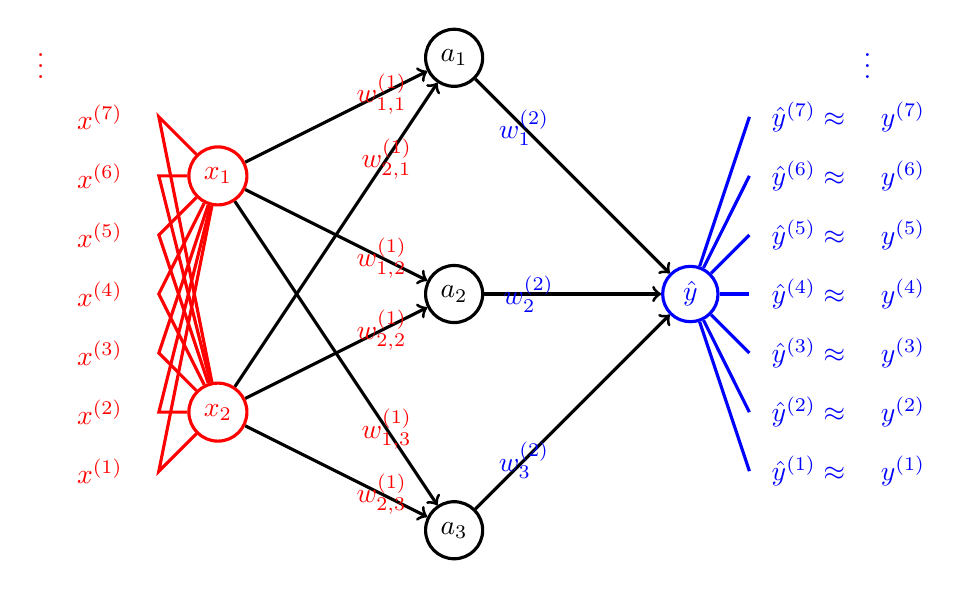
\begin{tikzpicture}[line width=0.4mm,minimum height=2em,scale=1.5]
  \node[draw,circle,red] (x1) at (0,1) {$x_1$};
  \node[draw,circle,red] (x2) at (0,-1) {$x_2$};
  \node[draw,circle] (a1) at (2,2) {$a_1$};
  \node[draw,circle] (a2) at (2,0) {$a_2$};
  \node[draw,circle] (a3) at (2,-2) {$a_3$};
  \node[draw,circle,blue] (y1) at (4,0) {$\hat{y}$};
  \foreach \x [count=\i] in {x1, x2} {
    \foreach \c [count=\j] in {a1, a2, a3} {
      \draw[->] (\x) -- (\c) node[red,near end] {$w^{(1)}_{\i,\j}$};
    }
  }
  \foreach \c [count=\i] in {a1, a2, a3} {
    \foreach \o in {y1} {
      \draw[->] (\c) -- (\o) node[blue,near start] {$w^{(2)}_{\i}$};
    }
  }
  \onslide<2->{
    \foreach \y [count=\i] in {-1.5,-1.0,...,1.5} {
      \node[red] at (-1.0,\y) {$x^{(\i)}$};
      \node[blue] at (5.8,\y) {$y^{(\i)}$};
      \pgfmathsetmacro{\j}{int(\i+2)}
      \onslide<\j>{
        \draw[red] (x1) -- (-0.5,\y) -- (x2);
        \draw[blue] (y1) -- (4.5,\y);
      }
      \onslide<\j->{
        \node[blue] at (5.0,\y) {$\hat{y}^{(\i)} \approx$};
      }
    }
    \node[red] at (-1.5,2.0) {$\vdots$};
    \node[blue] at (5.5,2.0) {$\vdots$};
  }
\end{tikzpicture}
\end{center}
}

\myframetop{
  \ctr{Redes Neurais}

  \[ E(W) = \frac{1}{2}\sum_{i=1}^m(y_i - \hat{y}_i(W))^2 \]

  \[ \min_W E(W) \]
}

\myframe{
  \ctr{Redes Neurais}
\begin{center}
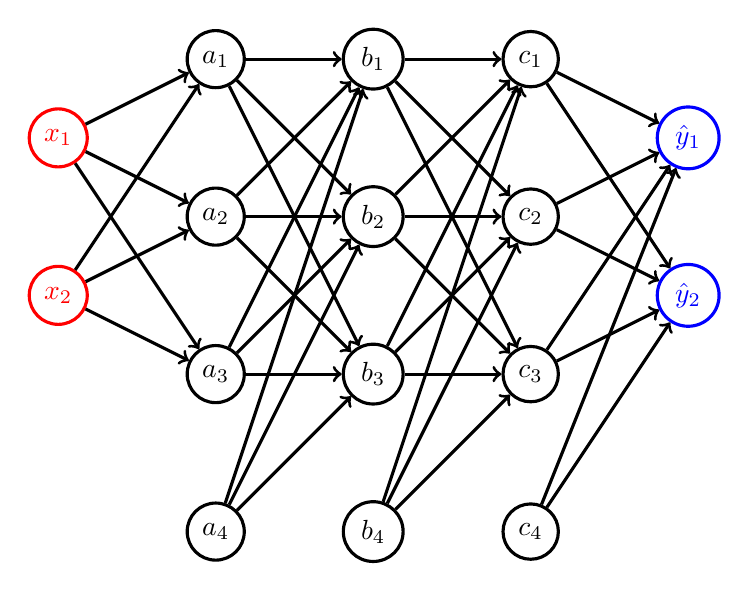
\begin{tikzpicture}[line width=0.4mm,minimum height=2em,scale=1.0]
  \node[draw,circle,red] (x1) at (0,1) {$x_1$};
  \node[draw,circle,red] (x2) at (0,-1) {$x_2$};
  \node[draw,circle] (a1) at (2,2) {$a_1$};
  \node[draw,circle] (a2) at (2,0) {$a_2$};
  \node[draw,circle] (a3) at (2,-2) {$a_3$};
  \node[draw,circle] (a4) at (2,-4) {$a_4$};
  \node[draw,circle] (b1) at (4,2) {$b_1$};
  \node[draw,circle] (b2) at (4,0) {$b_2$};
  \node[draw,circle] (b3) at (4,-2) {$b_3$};
  \node[draw,circle] (b4) at (4,-4) {$b_4$};
  \node[draw,circle] (c1) at (6,2) {$c_1$};
  \node[draw,circle] (c2) at (6,0) {$c_2$};
  \node[draw,circle] (c3) at (6,-2) {$c_3$};
  \node[draw,circle] (c4) at (6,-4) {$c_4$};
  \node[draw,circle,blue] (y1) at (8,1) {$\hat{y}_1$};
  \node[draw,circle,blue] (y2) at (8,-1) {$\hat{y}_2$};
  \foreach \x [count=\i] in {x1, x2} {
    \foreach \b [count=\j] in {a1, a2, a3} {
      \draw[->] (\x) -- (\b) node[red,near end] {};
    }
  }
  \foreach \b [count=\i] in {a1, a2, a3, a4} {
    \foreach \c [count=\j] in {b1, b2, b3} {
      \draw[->] (\b) -- (\c) node[red,near end] {};
    }
  }
  \foreach \b [count=\i] in {b1, b2, b3, b4} {
    \foreach \c [count=\j] in {c1, c2, c3} {
      \draw[->] (\b) -- (\c) node[red,near end] {};
    }
  }
  \foreach \c [count=\i] in {c1, c2, c3, c4} {
    \foreach \o [count=\j] in {y1, y2} {
      \draw[->] (\c) -- (\o) node[blue,near start] {};
    }
  }
\end{tikzpicture}
\end{center}
}

\myframe{
  \ctr{Exemplos}
  \begin{itemize}
    \item $x$ é uma imagem e $y$ é se tem um gato ou não;
    \item $x$ é uma imagem de uma palavra, e $y$ é a palavra (OCR e reCAPTCHA);
    \item $x$ é um tabuleiro, e $y$ é a próxima jogada.
  \end{itemize}
}

\myframe{
  \ctr{Em Go}
  \begin{itemize}
    \item Usa um banco de dados gigantesco para treinar;
    \item MCTS das melhores:
    \item Aumenta o banco de dados jogando com si mesmo:
    \item Projeto futuro: Não usar o banco de dados inicial.
  \end{itemize}
}

\subsection{Projetos}

\myframe{
  \ctr{Projetos}
  \begin{itemize}
    \item Estudar teoria de jogos;
    \item Estudar jogos educativos, ou gamificação da educação;
    \item Machine Learning com algum jogo simples, como Asteroids;
    \item Estudar Support Vector Machine, que cai em otimização;
    \item Algoritmos genéticos.
  \end{itemize}
}
